%
% ---------- header -----------------------------------------------------------
%
% project       kaneton
%
% license       kaneton
%
% file          /home/mycure/kaneton/view/book/assignments/k1.tex
%
% created       julien quintard   [fri nov 28 05:25:37 2008]
% updated       julien quintard   [mon may 17 15:29:10 2010]
%

%
% ---------- k1 ---------------------------------------------------------------
%

\chapter{k1}
\label{chapter:k1}

\name{k1} consists in the development of the memory management system.

\newpage

%
% ---------- text -------------------------------------------------------------
%

%
% objectives
%

\section{Objectives}

This project aims at learning advanced memory management in operating systems. Students will learn how to deal with MMU and Cache entries (TLB) through the concepts of Physical Memory, Virtual Memory and Address Space.

The students will also have to implement a memory allocator, with the algorithm of their choice.

%
% requirements
%

\section{Requirements}

The students must know the concepts of Physycal and Virtual memory and the mapping techniques. Especially the paging technique must be known since it is what has to be implemented. Since this implementation will be tested on the ia32 architecture, the students will need the Intel documentation so they can find how to interface with the MMU.

%
% snapshot
%

\section{Snapshot}

There are 4 main managers in the kaneton design that are used to handle memory :

\begin{itemize}
\item \textbf{segment :} In the kaneton terminology, a segment is a block of physical memory. The segment manager handles the allocation of blocks in the physical memory, provides methods to read and write these blocks, and to set permissions on these blocks. Please note that this is not related to the Intel segment concept.

\item \textbf{region :} In the kaneton terminology, a region is a block of virtual memory. The region manager handles the allocation of blocks in the virtual memory as well as the mapping of these blocks to kaneton segments, and provides methods to read, write, and set permissions on these blocks. Please note that the region manager will never reserve a segment by itself, allocating a region requires to provide a valid, already allocated, segment.

\item \textbf{map :} The map manager in kaneton is a higher level interface that handles memory allocation. It will reserve a segment, and will map a region on the segment with a single call.

\item \textbf{as :} The as manager is used to represent an address space (a set of regions mapped to segments, that belongs to a task).

\end{itemize}

%
% assignments
%

\section{Assignments}

\subsection*{Abstract}

The segment manager, the map manager and the as manager are already provided in the snapshot. The students will have to implement the region manager completely.

A region designs a block of virtual memory, so it is a quite generic concept. Some of the work to be done is therefore architecture dependant, but since it also consists in dealing with the MMU mappings, some part of it is architecture dependant.

Kaneton is a portable kernel, so each module has been designed to have an independant code (core) and several dependant code(machine), one for each architecture. The sudents will have to think about which code should go in the core or in the machine part. Please note that some functions may only have independant code.

\subsection*{Files}

\begin{tabular}{| l | l |}
  \hline
  machine-independent & {\em kaneton/core/region/region.c}\\\hline
  machine-dependent & {\em kaneton/machine/glue/ibm-pc.ia32/region.c}\\\hline
  machine-dependent & {\em kaneton/machine/architecture/ia32/paging.c}\\\hline
  machine-dependent & {\em kaneton/machine/architecture/ia32/pd.c}\\\hline
  machine-dependent & {\em kaneton/machine/architecture/ia32/pt.c}\\\hline
  machine-dependent & {\em kaneton/machine/architecture/ia32/tlb.c}\\\hline
  machine-dependent & {\em kaneton/machine/architecture/ia32/mapping.c}\\\hline
\end{tabular}

\subsection*{Required implementation}

\function{t\_error}{region\_initialize}{\type{t\_vaddr} \argument{start},
					\type{t\_vsize} \argument{size}}
{
  This function initializes the region manager. The virtual addresses that can
  be returned by the allocator must be in the range defined by \argument{start}
  and \argument{size}.
}

\function{t\_error}{region\_clean}{\type{void}}
{
  This function releases the ressources of the region manager.
}

\function{t\_error}{region\_reserve}{\type{i\_as} \argument{asid},
				     \type{i\_segment} \argument{segid},
				     \type{t\_paddr} \argument{offset},
				     \type{t\_opts} \argument{opts},
				     \type{t\_vaddr} \argument{address},
				     \type{t\_vsize} \argument{size},
				     \type{i\_region*} \argument{regid}}
{
  This function reserves a region of size \argument{size} in the address space
  \argument{asid} and maps the segment \argument{segid} to it. The identifier
  of this new region object is returned through the \argument{regid} parameter.
  
  \-
  
  The values for \argument{opts} can be:
  \begin{itemize}
    \item REGION\_OPT\_NONE: no options
    \item REGION\_OPT\_FORCE: force the region to be reserved at virtual
      address \argument{address}. Otherwise, it uses the algorithm of your choice to find a free address.
    \item REGION\_OPT\_USER: The region will be addressable both in the user
      and kernel mode.
    \item REGION\_OPT\_PRIVILEGED: The region will only be addressable in the
      kernel mode.
    \item REGION\_OPT\_LOCAL: The region will be local to the address space
      specified by \argument{asid}
    \item REGION\_OPT\_GLOBAL: The region will be global to all the address
      spaces.
  \end{itemize}
  \argument{offset} specifies the offset in the segment where the mapping of the region occurs, so that reserving several regions on the same segment is possible.
  \begin{center}
    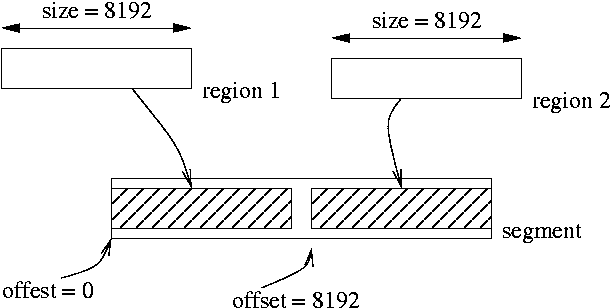
\includegraphics[width=0.4\linewidth]{figures/k1-offset}
  \end{center}

}

\function{t\_error}{region\_release}{\type{i\_as} \argument{asid},
				     \type{i\_region} \argument{regid}}
{
  This function releases the region \argument{regid} that belongs to the
  address space \argument{asid}.
}

\function{t\_error}{region\_inject}{\type{i\_as} \argument{asid},
                                    \type{o\_region*} \argument{o},
				    \type{i\_region*} \argument{regid}}
{
  This function injects the region \argument{o} into the address space
  \argument{asid}. 
}

\function{t\_error}{region\_flush}{\type{i\_as} \argument{asid}}
{
  This function releases all the regions of the address space \argument{asid}.
}

\function{t\_error}{region\_get}{\type{i\_as} \argument{asid},
				 \type{i\_region} \argument{regid},
				 \type{o\_region**} \argument{o}}
{
  This function returns the region object from its id \argument{regid} and the
  address space \argument{asid}, through the parameter \argument{o}.
}

\function{t\_error}{ia32\_pd\_activate}{\type{t\_ia32\_directory} \argument{dir},
                                        \type{t\_uint32} \argument{cached},
					\type{t\_uint32} \argument{writeback}}
{
  This function activates the page directory \argument{dir} by putting its
  address in the PDBR. The arguments \argument{cached} and \argument{writeback}
  control respectively if the cache should be enabled, or if the cache policy
  should be writeback. The flags of the PDBR register must be setup accordingly.
  
}

\function{t\_error}{ia32\_pd\_get\_cr3}{\type{t\_uint32*} \argument{cr3},
					\type{t\_ia32\_directory} \argument{dir},
					\type{t\_uint32} \argument{cached},
					\type{t\_uint32} \argument{writeback}}
{
  This function builds the value to put in the CR3 register to activate the page
  directory \argument{dir} with the \argument{cached} and \argument{writeback} flags
  set accordingly. The built value is returned in \argument{cr3}.
}

\function{t\_error}{ia32\_pd\_add\_table}{\type{t\_ia32\_directory*} \argument{dir},
					  \type{t\_uint16} \argument{entry},
					  \type{t\_ia32\_table} \argument{table}}
{
  This functions adds the page table \argument{table} in the page directory
  \argument{dir} at the index \argument{entry}.
}

\function{t\_error}{ia32\_pd\_get\_table}{\type{t\_ia32\_directory*} \argument{dir},
					  \type{t\_uint16} \argument{entry},
					  \type{t\_ia32\_table*} \argument{table}}
{
  This functions gets the page table \argument{table} from the page directory
  \argument{dir} at the index \argument{entry}.
}

\function{t\_error}{ia32\_pd\_delete\_table}{\type{t\_ia32\_directory*} \argument{dir},
					     \type{t\_uint16} \argument{entry}}
{
  This functions removes the page table at the index \argument{entry} from the
  page directory \argument{dir}.
}

\function{t\_error}{ia32\_pt\_build}{\type{t\_paddr} \argument{base},
				     \type{t\_ia32\_table*} \argument{table}}
{
  This function initializes the page table entry \argument{table} with the
  physical address \argument{base}
}

\function{t\_error}{ia32\_pt\_add\_page}{\type{t\_ia32\_table*} \argument{tab},
					 \type{t\_uint16} \argument{entry},
					 \type{t\_ia32\_page} \argument{page}}
{
  This functions adds the page \argument{page} in the page table
  \argument{tab} at the index \argument{entry}.
}

\function{t\_error}{ia32\_pt\_get\_page}{\type{t\_ia32\_table*} \argument{tab},
					 \type{t\_uint16} \argument{entry},
					 \type{t\_ia32\_page*} \argument{page}}
{
  This functions gets the page \argument{page} from the page table
  \argument{tab} at the index \argument{entry}.
}

\function{t\_error}{ia32\_pt\_delete\_page}{\type{t\_ia32\_table*} \argument{tab},
					    \type{t\_uint16} \argument{entry}}
{
  This functions removes the page at the index \argument{entry} from the
  page table \argument{tab}.
}

\function{t\_error}{ia32\_tlb\_invalidate}{\type{t\_vaddr} \argument{page}}
{
  This functions invalidates the TLB entry for the virual address
  \argument{page}.
}

\function{t\_error}{ia32\_tlb\_flush}{\type{void}}
{
  This functions flushes the TLB of the CPU.
}

\function{t\_error}{ia32\_map\_pd}{\type{t\_ia32\_directory*} \argument{pd}}
{
  This function takes the physical address of a page directory in \argument{pd}.
  It will map this page directory in the kernel address space, and return
  the virtual address by erasing the content of \argument{pd}.
  The type of the argument is a physical address, not a virtual address, but
  since they are both 32-bit values, you can just cast your virtual address
  to put it in the value pointed by \argument{pd}.
  In other words, when the function is called, it takes a physical address of
  a page directory in the memory space pointed by \argument{pd}, the function
  should then map this page directory, and the virtual address which has been
  assigned for this mapping should be put in the memory space pointed by
  \argument{pd} even though its type doesn't represent a virtual address.
}

\function{t\_error}{ia32\_map\_pt}{\type{t\_ia32\_table*} \argument{pt}}
{
  This function takes a page table structure in \argument{pt}. It will retrieve
  the physical address of this page from this struct, map it in the kernel address
  space, and return the virtual address through the appropriate field of this
  struct \argument{pt}.
}

\function{t\_error}{ia32\_map\_region}{\type{i\_as} \argument{asid},
                                       \type{i\_segment} \argument{segid},
				       \type{t\_paddr} \argument{offset},
				       \type{t\_opts} \argument{opts},
				       \type{t\_vaddr} \argument{address},
				       \type{t\_vsize} \argument{size}}
{
  This function will map the region defined by \argument{address} and \argument{size}
  on the segment defined by \argument{segid} at the offset \argument{offset}, in the
  address space defined by \argument{asid}.
  
  \-

  The \argument{opts} are similar to \emph{region\_reserve}.

  \-

  Refer to the figure in the \emph{region\_reserve} description to understand what
  \argument{offset} is used for.

  \-

  This function will create page tables if required.
}

\function{t\_error}{ia32\_unmap\_region}{\type{i\_as} \argument{asid},
					 \type{t\_vaddr} \argument{address},
					 \type{t\_vsize} \argument{size}}
{
  This function will unmap the region defined by \argument{address} and \argument{size}
  from the address space defined by \argument{asid}.

  \-

  This function must release the memory of page tables that gets empty upon unmapping.
}

\subsection*{Optional implementation}

The following functions are not going to be tested by our test suite, you are
not forced to do them although we strongly recommend you to do it, since they
are very helpful for debugging your implementation.

\-

Since this is not tested, the output format is up to you.

\function{t\_error}{region\_show}{\type{i\_as} \argument{asid},
                                  \type{i\_region} \argument{regid}}
{
  This function displays the region object specified by its id \argument{regid}
  and the address space \argument{asid}.
}

\function{t\_error}{region\_dump}{\type{i\_as} \argument{asid}}
{
  This function displays all the region objects that belong to the address
  space \argument{asid}.
}

\function{t\_error}{ia32\_pd\_dump}{\type{t\_ia32\_directory*} \argument{dir}}
{
  This function displays the content of the page directory \argument{dir}.
}

\function{t\_error}{ia32\_pt\_dump}{\type{t\_ia32\_pte*} \argument{tab}}
{
  This function displays the content of the page table \argument{dir}.
}

\subsection*{Important}
Please note that you have the core and the machine part to do.
All the functions might not require a machine part though. The machine
part file (glue) doesn't contain any prototypes.
It's your responsability to add a machine function, in glue if you think
it needs one.

\-

In the machine part, we also removed some full functions (including the prototypes). You are free to make new functions, to make your code cleaner, as long as you at least implement the required interface below.

\-

Some structures relative to the region manager are already provided, but you
are free to modify them if you want to. You can freely add new fields, and also
modify the existing ones, but in that case, it's your responsibility to make
changes in the code so that everything still works.
